\documentclass[twoside]{book}

% Packages required by doxygen
\usepackage{fixltx2e}
\usepackage{calc}
\usepackage{doxygen}
\usepackage{graphicx}
\usepackage[utf8]{inputenc}
\usepackage{makeidx}
\usepackage{multicol}
\usepackage{multirow}
\PassOptionsToPackage{warn}{textcomp}
\usepackage{textcomp}
\usepackage[nointegrals]{wasysym}
\usepackage[table]{xcolor}

% Font selection
\usepackage[T1]{fontenc}
\usepackage{mathptmx}
\usepackage[scaled=.90]{helvet}
\usepackage{courier}
\usepackage{amssymb}
\usepackage{sectsty}
\renewcommand{\familydefault}{\sfdefault}
\allsectionsfont{%
  \fontseries{bc}\selectfont%
  \color{darkgray}%
}
\renewcommand{\DoxyLabelFont}{%
  \fontseries{bc}\selectfont%
  \color{darkgray}%
}
\newcommand{\+}{\discretionary{\mbox{\scriptsize$\hookleftarrow$}}{}{}}

% Page & text layout
\usepackage{geometry}
\geometry{%
  a4paper,%
  top=2.5cm,%
  bottom=2.5cm,%
  left=2.5cm,%
  right=2.5cm%
}
\tolerance=750
\hfuzz=15pt
\hbadness=750
\setlength{\emergencystretch}{15pt}
\setlength{\parindent}{0cm}
\setlength{\parskip}{0.2cm}
\makeatletter
\renewcommand{\paragraph}{%
  \@startsection{paragraph}{4}{0ex}{-1.0ex}{1.0ex}{%
    \normalfont\normalsize\bfseries\SS@parafont%
  }%
}
\renewcommand{\subparagraph}{%
  \@startsection{subparagraph}{5}{0ex}{-1.0ex}{1.0ex}{%
    \normalfont\normalsize\bfseries\SS@subparafont%
  }%
}
\makeatother

% Headers & footers
\usepackage{fancyhdr}
\pagestyle{fancyplain}
\fancyhead[LE]{\fancyplain{}{\bfseries\thepage}}
\fancyhead[CE]{\fancyplain{}{}}
\fancyhead[RE]{\fancyplain{}{\bfseries\leftmark}}
\fancyhead[LO]{\fancyplain{}{\bfseries\rightmark}}
\fancyhead[CO]{\fancyplain{}{}}
\fancyhead[RO]{\fancyplain{}{\bfseries\thepage}}
\fancyfoot[LE]{\fancyplain{}{}}
\fancyfoot[CE]{\fancyplain{}{}}
\fancyfoot[RE]{\fancyplain{}{\bfseries\scriptsize Generated on Wed Dec 10 2014 01\+:15\+:35 for C\+A\+L\+C\+U\+L\+A\+T\+O\+R by Doxygen }}
\fancyfoot[LO]{\fancyplain{}{\bfseries\scriptsize Generated on Wed Dec 10 2014 01\+:15\+:35 for C\+A\+L\+C\+U\+L\+A\+T\+O\+R by Doxygen }}
\fancyfoot[CO]{\fancyplain{}{}}
\fancyfoot[RO]{\fancyplain{}{}}
\renewcommand{\footrulewidth}{0.4pt}
\renewcommand{\chaptermark}[1]{%
  \markboth{#1}{}%
}
\renewcommand{\sectionmark}[1]{%
  \markright{\thesection\ #1}%
}

% Indices & bibliography
\usepackage{natbib}
\usepackage[titles]{tocloft}
\setcounter{tocdepth}{3}
\setcounter{secnumdepth}{5}
\makeindex

% Hyperlinks (required, but should be loaded last)
\usepackage{ifpdf}
\ifpdf
  \usepackage[pdftex,pagebackref=true]{hyperref}
\else
  \usepackage[ps2pdf,pagebackref=true]{hyperref}
\fi
\hypersetup{%
  colorlinks=true,%
  linkcolor=blue,%
  citecolor=blue,%
  unicode%
}

% Custom commands
\newcommand{\clearemptydoublepage}{%
  \newpage{\pagestyle{empty}\cleardoublepage}%
}


%===== C O N T E N T S =====

\begin{document}

% Titlepage & ToC
\hypersetup{pageanchor=false,
             bookmarks=true,
             bookmarksnumbered=true,
             pdfencoding=unicode
            }
\pagenumbering{roman}
\begin{titlepage}
\vspace*{7cm}
\begin{center}%
{\Large C\+A\+L\+C\+U\+L\+A\+T\+O\+R }\\
\vspace*{1cm}
{\large Generated by Doxygen 1.8.8}\\
\vspace*{0.5cm}
{\small Wed Dec 10 2014 01:15:35}\\
\end{center}
\end{titlepage}
\clearemptydoublepage
\tableofcontents
\clearemptydoublepage
\pagenumbering{arabic}
\hypersetup{pageanchor=true}

%--- Begin generated contents ---
\chapter{Developing-\/\+Computer-\/\+Programming-\/\+Program-\/\+Elements-\/\+Structure}
\label{md__last_badge__developing_computer_programming__r_e_a_d_m_e}
\hypertarget{md__last_badge__developing_computer_programming__r_e_a_d_m_e}{}
Developing Computer Programming\+: Program Elements \& Structure, challenges, programs and documentation

The repository master branch has the Expression\+Calc program divided into two parts. The function \hyperlink{_bitwise_8c_a1069f717b1478dfc4f451a08a1690884}{Bitwise()} has been declared in \hyperlink{_bitwise_8h}{Bitwise.\+h} and defined in \hyperlink{_bitwise_8c}{Bitwise.\+c} A Makefile is also used to tell the complier about the different source files. The rest of the documentation can be found in the index.\+html Doxygen folder. 
\chapter{File Index}
\section{File List}
Here is a list of all files with brief descriptions\+:\begin{DoxyCompactList}
\item\contentsline{section}{Last\+Badge/\+Developing\+Computer\+Programming/\hyperlink{_bitwise_8c}{Bitwise.\+c} }{\pageref{_bitwise_8c}}{}
\item\contentsline{section}{Last\+Badge/\+Developing\+Computer\+Programming/\hyperlink{_bitwise_8h}{Bitwise.\+h} }{\pageref{_bitwise_8h}}{}
\item\contentsline{section}{Last\+Badge/\+Developing\+Computer\+Programming/\hyperlink{_expression_calc_8c}{Expression\+Calc.\+c} }{\pageref{_expression_calc_8c}}{}
\end{DoxyCompactList}

\chapter{File Documentation}
\hypertarget{_bitwise_8c}{\section{Last\+Badge/\+Developing\+Computer\+Programming/\+Bitwise.c File Reference}
\label{_bitwise_8c}\index{Last\+Badge/\+Developing\+Computer\+Programming/\+Bitwise.\+c@{Last\+Badge/\+Developing\+Computer\+Programming/\+Bitwise.\+c}}
}
{\ttfamily \#include \char`\"{}Bitwise.\+h\char`\"{}}\\*
{\ttfamily \#include $<$stdio.\+h$>$}\\*
Include dependency graph for Bitwise.\+c\+:
\nopagebreak
\begin{figure}[H]
\begin{center}
\leavevmode
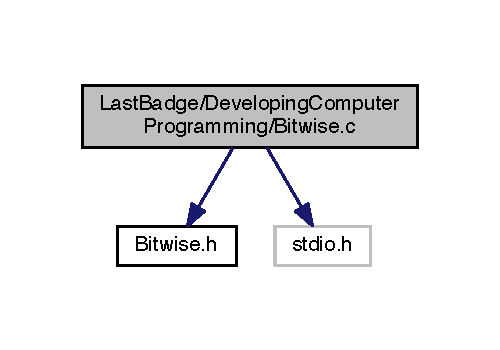
\includegraphics[width=240pt]{_bitwise_8c__incl}
\end{center}
\end{figure}
\subsection*{Functions}
\begin{DoxyCompactItemize}
\item 
void \hyperlink{_bitwise_8c_a1069f717b1478dfc4f451a08a1690884}{Bitwise} ()
\begin{DoxyCompactList}\small\item\em Calculator. \end{DoxyCompactList}\end{DoxyCompactItemize}


\subsection{Function Documentation}
\hypertarget{_bitwise_8c_a1069f717b1478dfc4f451a08a1690884}{\index{Bitwise.\+c@{Bitwise.\+c}!Bitwise@{Bitwise}}
\index{Bitwise@{Bitwise}!Bitwise.\+c@{Bitwise.\+c}}
\subsubsection[{Bitwise}]{\setlength{\rightskip}{0pt plus 5cm}void Bitwise (
\begin{DoxyParamCaption}
{}
\end{DoxyParamCaption}
)}}\label{_bitwise_8c_a1069f717b1478dfc4f451a08a1690884}


Calculator. 





\begin{DoxyAuthor}{Author}
Nishant Jain
\end{DoxyAuthor}
\begin{DoxyDate}{Date}
9 December 2014
\end{DoxyDate}
A source file with function \hyperlink{_bitwise_8c_a1069f717b1478dfc4f451a08a1690884}{Bitwise()}





Bitwise

\begin{DoxyAuthor}{Author}
Nishant Jain
\end{DoxyAuthor}
\begin{DoxyDate}{Date}
November 27, 2014
\end{DoxyDate}
This function uses and displays bit operations on variables

Required Files/\+Databases\+: None

Non System Routines Called\+: None

Return Value\+: None

O\+S Specific Assumptions\+: None

Local Variables\+: A integer used for calculating sum B integer used in for loop C integer used to calulate sum 

Definition at line 45 of file Bitwise.\+c.



Referenced by Extra().


\begin{DoxyCode}
46 \{
47   \textcolor{keywordtype}{int} A, B, C;
48   printf(\textcolor{stringliteral}{"Type two integers to learn about bitwise operations. A= "});
49   scanf(\textcolor{stringliteral}{" %d"}, &A);
50   printf(\textcolor{stringliteral}{"\(\backslash\)n B= "});
51   scanf(\textcolor{stringliteral}{" %d"}, &B);
52   C= A & B;
53   printf(\textcolor{stringliteral}{"AND: A & B = %d \(\backslash\)n"}, C);
54   C= A | B;
55   printf(\textcolor{stringliteral}{"OR: A | B = %d \(\backslash\)n"}, C);
56   C= A ^ B;
57   printf(\textcolor{stringliteral}{"XOR: A ^ B = %d \(\backslash\)n"}, C);
58   C= ~A;
59   printf(\textcolor{stringliteral}{"COMPLEMENT: ~A = %d \(\backslash\)n"}, C);
60   C= A <<2;
61   printf(\textcolor{stringliteral}{"LESFT SHIFT: A <<2 = %d \(\backslash\)n"}, C);
62   C= A >>2;
63   printf(\textcolor{stringliteral}{"RIGHT SHIFT: A >>2 = %d \(\backslash\)n"}, C);
64 
65 \}\end{DoxyCode}


Here is the caller graph for this function\+:
\nopagebreak
\begin{figure}[H]
\begin{center}
\leavevmode
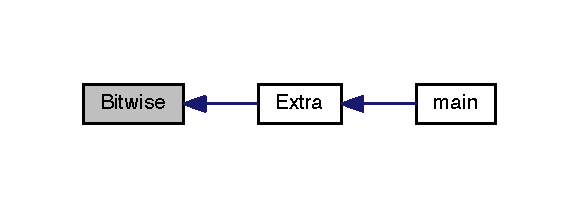
\includegraphics[width=278pt]{_bitwise_8c_a1069f717b1478dfc4f451a08a1690884_icgraph}
\end{center}
\end{figure}



\hypertarget{_bitwise_8h}{\section{Last\+Badge/\+Developing\+Computer\+Programming/\+Bitwise.h File Reference}
\label{_bitwise_8h}\index{Last\+Badge/\+Developing\+Computer\+Programming/\+Bitwise.\+h@{Last\+Badge/\+Developing\+Computer\+Programming/\+Bitwise.\+h}}
}
This graph shows which files directly or indirectly include this file\+:
\nopagebreak
\begin{figure}[H]
\begin{center}
\leavevmode
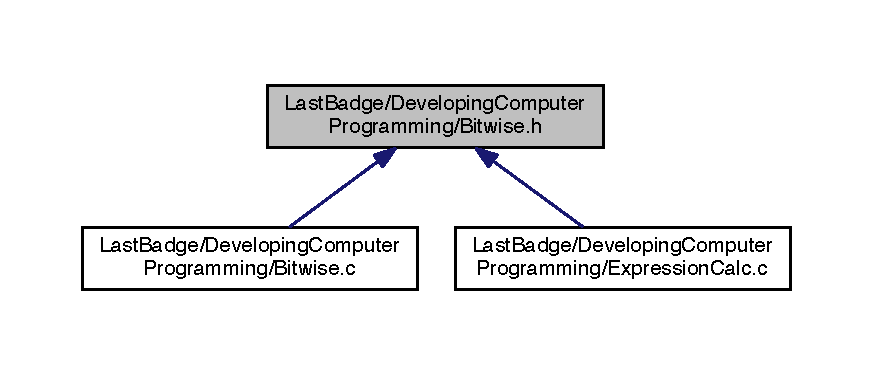
\includegraphics[width=350pt]{_bitwise_8h__dep__incl}
\end{center}
\end{figure}
\subsection*{Functions}
\begin{DoxyCompactItemize}
\item 
void \hyperlink{_bitwise_8h_a1069f717b1478dfc4f451a08a1690884}{Bitwise} ()
\begin{DoxyCompactList}\small\item\em Calculator. \end{DoxyCompactList}\end{DoxyCompactItemize}


\subsection{Function Documentation}
\hypertarget{_bitwise_8h_a1069f717b1478dfc4f451a08a1690884}{\index{Bitwise.\+h@{Bitwise.\+h}!Bitwise@{Bitwise}}
\index{Bitwise@{Bitwise}!Bitwise.\+h@{Bitwise.\+h}}
\subsubsection[{Bitwise}]{\setlength{\rightskip}{0pt plus 5cm}void Bitwise (
\begin{DoxyParamCaption}
{}
\end{DoxyParamCaption}
)}}\label{_bitwise_8h_a1069f717b1478dfc4f451a08a1690884}


Calculator. 





\begin{DoxyAuthor}{Author}
Nishant Jain
\end{DoxyAuthor}
\begin{DoxyDate}{Date}
9 December 2014
\end{DoxyDate}
A source file with function \hyperlink{_bitwise_8c_a1069f717b1478dfc4f451a08a1690884}{Bitwise()}





Bitwise

\begin{DoxyAuthor}{Author}
Nishant Jain
\end{DoxyAuthor}
\begin{DoxyDate}{Date}
November 27, 2014
\end{DoxyDate}
This function uses and displays bit operations on variables

Required Files/\+Databases\+: None

Non System Routines Called\+: None

Return Value\+: None

O\+S Specific Assumptions\+: None

Local Variables\+: A integer used for calculating sum B integer used in for loop C integer used to calulate sum 

Definition at line 45 of file Bitwise.\+c.



Referenced by Extra().


\begin{DoxyCode}
46 \{
47   \textcolor{keywordtype}{int} A, B, C;
48   printf(\textcolor{stringliteral}{"Type two integers to learn about bitwise operations. A= "});
49   scanf(\textcolor{stringliteral}{" %d"}, &A);
50   printf(\textcolor{stringliteral}{"\(\backslash\)n B= "});
51   scanf(\textcolor{stringliteral}{" %d"}, &B);
52   C= A & B;
53   printf(\textcolor{stringliteral}{"AND: A & B = %d \(\backslash\)n"}, C);
54   C= A | B;
55   printf(\textcolor{stringliteral}{"OR: A | B = %d \(\backslash\)n"}, C);
56   C= A ^ B;
57   printf(\textcolor{stringliteral}{"XOR: A ^ B = %d \(\backslash\)n"}, C);
58   C= ~A;
59   printf(\textcolor{stringliteral}{"COMPLEMENT: ~A = %d \(\backslash\)n"}, C);
60   C= A <<2;
61   printf(\textcolor{stringliteral}{"LESFT SHIFT: A <<2 = %d \(\backslash\)n"}, C);
62   C= A >>2;
63   printf(\textcolor{stringliteral}{"RIGHT SHIFT: A >>2 = %d \(\backslash\)n"}, C);
64 
65 \}\end{DoxyCode}


Here is the caller graph for this function\+:
\nopagebreak
\begin{figure}[H]
\begin{center}
\leavevmode
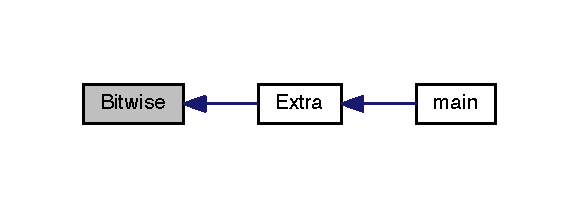
\includegraphics[width=278pt]{_bitwise_8h_a1069f717b1478dfc4f451a08a1690884_icgraph}
\end{center}
\end{figure}



\hypertarget{_expression_calc_8c}{\section{Last\+Badge/\+Developing\+Computer\+Programming/\+Expression\+Calc.c File Reference}
\label{_expression_calc_8c}\index{Last\+Badge/\+Developing\+Computer\+Programming/\+Expression\+Calc.\+c@{Last\+Badge/\+Developing\+Computer\+Programming/\+Expression\+Calc.\+c}}
}
{\ttfamily \#include $<$stdio.\+h$>$}\\*
{\ttfamily \#include $<$stdlib.\+h$>$}\\*
{\ttfamily \#include $<$math.\+h$>$}\\*
{\ttfamily \#include \char`\"{}Bitwise.\+h\char`\"{}}\\*
Include dependency graph for Expression\+Calc.\+c\+:
\nopagebreak
\begin{figure}[H]
\begin{center}
\leavevmode
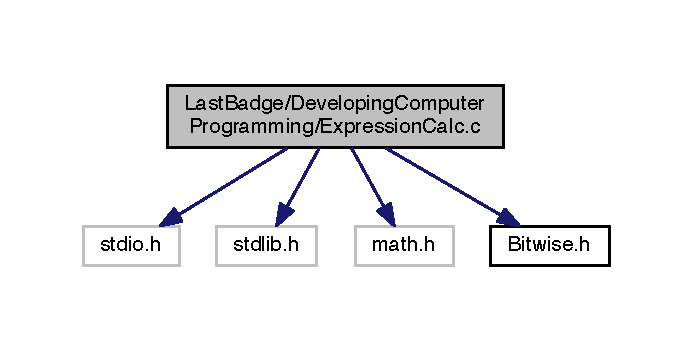
\includegraphics[width=332pt]{_expression_calc_8c__incl}
\end{center}
\end{figure}
\subsection*{Functions}
\begin{DoxyCompactItemize}
\item 
void \hyperlink{_expression_calc_8c_a79cd2ba7236d8017474e3340e169f888}{Extra} ()
\begin{DoxyCompactList}\small\item\em Calculator. \end{DoxyCompactList}\item 
void \hyperlink{_expression_calc_8c_a1f044085ede204d3d2ba2e4db44e7e5d}{Calc\+Fib} (int r)
\begin{DoxyCompactList}\small\item\em Calc\+Fib. \end{DoxyCompactList}\item 
int \hyperlink{_expression_calc_8c_ae66f6b31b5ad750f1fe042a706a4e3d4}{main} ()
\begin{DoxyCompactList}\small\item\em main \end{DoxyCompactList}\end{DoxyCompactItemize}


\subsection{Function Documentation}
\hypertarget{_expression_calc_8c_a1f044085ede204d3d2ba2e4db44e7e5d}{\index{Expression\+Calc.\+c@{Expression\+Calc.\+c}!Calc\+Fib@{Calc\+Fib}}
\index{Calc\+Fib@{Calc\+Fib}!Expression\+Calc.\+c@{Expression\+Calc.\+c}}
\subsubsection[{Calc\+Fib}]{\setlength{\rightskip}{0pt plus 5cm}void Calc\+Fib (
\begin{DoxyParamCaption}
\item[{int}]{r}
\end{DoxyParamCaption}
)}}\label{_expression_calc_8c_a1f044085ede204d3d2ba2e4db44e7e5d}


Calc\+Fib. 





\begin{DoxyAuthor}{Author}
Nishant Jain
\end{DoxyAuthor}
\begin{DoxyDate}{Date}
November 27, 2014
\end{DoxyDate}
function finds sum of Fibonacci Series

Required Files/\+Databases\+: None

Non System Routines Called\+: None

Return Value\+: None

O\+S Specific Assumptions\+: None

Local Variables\+: j integer used for calculating sum i integer used in for loop k integer used to calulate sum res integer used to calulate sum sum long integer to store sum of fibonacci series 

Definition at line 253 of file Expression\+Calc.\+c.



Referenced by Extra().


\begin{DoxyCode}
254 \{
255   \textcolor{keywordtype}{int} j=0, i=2, k=1, res;
256   \textcolor{keywordtype}{long} \textcolor{keywordtype}{int} sum=1;
257   
258   printf(\textcolor{stringliteral}{"FIBONACCI SERIES: "});
259   \textcolor{comment}{//printing first two values.}
260   printf(\textcolor{stringliteral}{"%d %d"},j,k); 
261 
262   \textcolor{comment}{/*}
263 \textcolor{comment}{  * Using increment operator in for loop}
264 \textcolor{comment}{  * Displaying Fibonacci series}
265 \textcolor{comment}{  * Using "+=" operator}
266 \textcolor{comment}{  * Finding Sum of Fibonacci series}
267 \textcolor{comment}{  */}
268   
269   \textcolor{keywordflow}{for}(i=2;i<r;i++)
270   \{
271     res=j+k;
272     j=k;
273     k=res; 
274     printf(\textcolor{stringliteral}{" %d"},k);
275     sum+=k;
276   \}  
277   printf(\textcolor{stringliteral}{"\(\backslash\)nSum of Fibonacci series= %ld \(\backslash\)n"}, sum); 
278 \}
\end{DoxyCode}


Here is the caller graph for this function\+:
\nopagebreak
\begin{figure}[H]
\begin{center}
\leavevmode
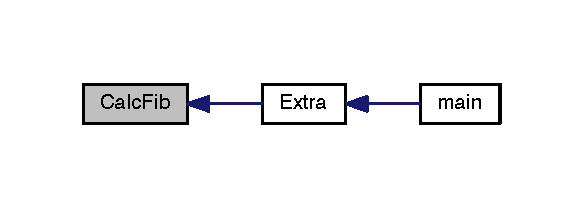
\includegraphics[width=280pt]{_expression_calc_8c_a1f044085ede204d3d2ba2e4db44e7e5d_icgraph}
\end{center}
\end{figure}


\hypertarget{_expression_calc_8c_a79cd2ba7236d8017474e3340e169f888}{\index{Expression\+Calc.\+c@{Expression\+Calc.\+c}!Extra@{Extra}}
\index{Extra@{Extra}!Expression\+Calc.\+c@{Expression\+Calc.\+c}}
\subsubsection[{Extra}]{\setlength{\rightskip}{0pt plus 5cm}void Extra (
\begin{DoxyParamCaption}
{}
\end{DoxyParamCaption}
)}}\label{_expression_calc_8c_a79cd2ba7236d8017474e3340e169f888}


Calculator. 

Extra.





\begin{DoxyAuthor}{Author}
Nishant Jain
\end{DoxyAuthor}
\begin{DoxyDate}{Date}
25 November 2014
\end{DoxyDate}
A Calulator program with basic Arithmetic Operations and some extra features such as sum of Fibonacci series, bitwise operations and square-\/root function



 \begin{DoxyAuthor}{Author}
Nishant Jain
\end{DoxyAuthor}
\begin{DoxyDate}{Date}
November 27, 2014
\end{DoxyDate}
This function calculates square root. Calls \hyperlink{_expression_calc_8c_a1f044085ede204d3d2ba2e4db44e7e5d}{Calc\+Fib()} and \hyperlink{_bitwise_8c_a1069f717b1478dfc4f451a08a1690884}{Bitwise()}

Required Files/\+Databases\+: None

Non System Routines Called\+: None

Return Value\+: None

O\+S Specific Assumptions\+: None

Local Variables\+: ch integer User's choice for operation r integer Parameter passed as range of fibonacci series sq float Square root of input number 

Definition at line 194 of file Expression\+Calc.\+c.



References Bitwise(), and Calc\+Fib().



Referenced by main().


\begin{DoxyCode}
195 \{ 
196   \textcolor{keywordtype}{int} ch,r;
197   \textcolor{keywordtype}{float} sq;
198 
199   printf(\textcolor{stringliteral}{"\(\backslash\)nSelect from the following options: \(\backslash\)n1)Fibonacci Series"}
200   \textcolor{stringliteral}{" \(\backslash\)n2)Bitwise Operations \(\backslash\)n3)Square root \(\backslash\)n"});
201   scanf(\textcolor{stringliteral}{" %d"},&ch);
202   
203   \textcolor{keywordflow}{switch}(ch)
204   \{
205     \textcolor{keywordflow}{case} 1:
206     printf(\textcolor{stringliteral}{"\(\backslash\)nEnter the range of Fibonacci series: \(\backslash\)n "}); 
207     scanf(\textcolor{stringliteral}{" %d"},&r);
208     \hyperlink{_expression_calc_8c_a1f044085ede204d3d2ba2e4db44e7e5d}{CalcFib}(r); \textcolor{keywordflow}{break};
209     
210     \textcolor{keywordflow}{case} 2:
211     \hyperlink{_bitwise_8c_a1069f717b1478dfc4f451a08a1690884}{Bitwise}(); \textcolor{keywordflow}{break};
212 
213     \textcolor{keywordflow}{case} 3:
214     printf(\textcolor{stringliteral}{"Enter the number you want the square root of: "});
215     scanf(\textcolor{stringliteral}{" %f"},&sq);
216     printf(\textcolor{stringliteral}{"\(\backslash\)n Square root of %f: "},sq); 
217     sq=sqrt(sq);
218     printf(\textcolor{stringliteral}{"%f"},sq);  \textcolor{keywordflow}{break};
219   \}
220 \}
\end{DoxyCode}


Here is the call graph for this function\+:
\nopagebreak
\begin{figure}[H]
\begin{center}
\leavevmode
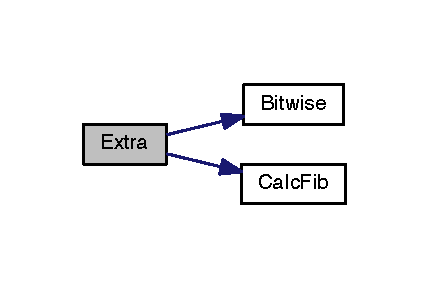
\includegraphics[width=206pt]{_expression_calc_8c_a79cd2ba7236d8017474e3340e169f888_cgraph}
\end{center}
\end{figure}




Here is the caller graph for this function\+:
\nopagebreak
\begin{figure}[H]
\begin{center}
\leavevmode
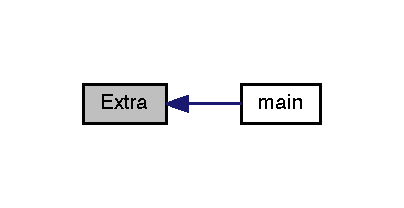
\includegraphics[width=194pt]{_expression_calc_8c_a79cd2ba7236d8017474e3340e169f888_icgraph}
\end{center}
\end{figure}


\hypertarget{_expression_calc_8c_ae66f6b31b5ad750f1fe042a706a4e3d4}{\index{Expression\+Calc.\+c@{Expression\+Calc.\+c}!main@{main}}
\index{main@{main}!Expression\+Calc.\+c@{Expression\+Calc.\+c}}
\subsubsection[{main}]{\setlength{\rightskip}{0pt plus 5cm}int main (
\begin{DoxyParamCaption}
{}
\end{DoxyParamCaption}
)}}\label{_expression_calc_8c_ae66f6b31b5ad750f1fe042a706a4e3d4}


main 





\begin{DoxyAuthor}{Author}
Nishant
\end{DoxyAuthor}
\begin{DoxyDate}{Date}
November 25, 2014
\end{DoxyDate}
Calls arithmetic functions and uses file to log outputs

Required Files/\+Databases\+: Log.\+txt

Non System Routines Called\+: None

Return Value\+: Type Description int return(0)

O\+S Specific Assumptions\+: None

Local Variables\+: Name Type Description check char To see if user wants to continue ch int User's choice of operation opt char User's choice of getting value from log file var1 float Operand 1 var2 float Operand 2 res float Result of Arithmetic operation

Modification History\+: Date Developer Action 8/20/2004 Jane Doe Changed the equation used to convert Celsius to Fahrenheit.

1 while loop 2 if-\/ else selection (N\+E\+S\+T\+E\+D) 2 switch-\/case constructs 1 for loop Flowchart diagram\+: 

An optional starting asterisk or space indicates that the data is to be read from the stream but ignored, i.\+e. it is not stored in the corresponding argument. Input of variable2

Definition at line 70 of file Expression\+Calc.\+c.



References Extra().


\begin{DoxyCode}
71 \{
72   \textcolor{comment}{//Welcome Screen}
73   printf(\textcolor{stringliteral}{"Welcome to Calculator. \(\backslash\)n"});
79   \textcolor{keywordtype}{char} check=\textcolor{charliteral}{'y'};
80   \textcolor{keywordtype}{int} ch;
81   \textcolor{keywordtype}{char} opt;
82   \textcolor{keywordtype}{float} var1, var2;
83   \textcolor{keywordtype}{float} res;
84   FILE * Log;
85 
86   \textcolor{comment}{//Opening a new file for Logging info. Opening in reading and writing mode}
87   Log = fopen (\textcolor{stringliteral}{"Log.txt"}, \textcolor{stringliteral}{"w+"});
88       
89   \textcolor{keywordflow}{while}(check!=\textcolor{charliteral}{'n'})
90   \{ 
91     printf(\textcolor{stringliteral}{"Please select an Arithmetic operation from the following:\(\backslash\)n"});
92     printf(\textcolor{stringliteral}{"1)Addition \(\backslash\)t 2)Subtraction \(\backslash\)t 3)Multiplication \(\backslash\)n4)Division"}
93     \textcolor{stringliteral}{"\(\backslash\)t 5)Power \(\backslash\)t 6)Extra Features \(\backslash\)n"});
94     
95     \textcolor{comment}{//Input of operation, A SPACE before %d makes scanf ignore whitespace}
96     scanf(\textcolor{stringliteral}{" %d"}, &ch);
97     
98     \textcolor{comment}{//Condition for Extra Features option}
99     \textcolor{keywordflow}{if}(ch!=6)
100     \{
101       \textcolor{comment}{//Asking user if he wants to use saved previous result}
102       printf(\textcolor{stringliteral}{"Do you want to use the previous result as"}
103         \textcolor{stringliteral}{" one of the operands (Y/N)? \(\backslash\)n"});
104       scanf(\textcolor{stringliteral}{" %c"}, &opt);
105       printf(\textcolor{stringliteral}{"Enter any values for operand(s): \(\backslash\)n"});
106       
107       \textcolor{keywordflow}{if}(opt==\textcolor{charliteral}{'Y'} || opt==\textcolor{charliteral}{'y'})
108       \{
109         printf(\textcolor{stringliteral}{"Operand 1 is the previous result: "});
110         rewind(Log);
111         \textcolor{comment}{//Taking value from the LOG text file for variable 1}
112         fscanf(Log, \textcolor{stringliteral}{" %f"}, &var1);
113         printf(\textcolor{stringliteral}{"%f \(\backslash\)n"}, var1);
114       \}  
115     
116       \textcolor{keywordflow}{else} 
117       \{
118         printf(\textcolor{stringliteral}{"Operand 1: "}); 
119         scanf(\textcolor{stringliteral}{"%f"}, &var1);
120       \}
121       
122       printf(\textcolor{stringliteral}{"Operand 2: "}); 
129       scanf(\textcolor{stringliteral}{" %f"}, &var2);
130       
131       \textcolor{comment}{//Switch case construct: Statements for different conditions }
132       \textcolor{keywordflow}{switch}(ch) 
133       \{
134         \textcolor{keywordflow}{case} 1: res=var1+var2; \textcolor{keywordflow}{break};
135         \textcolor{keywordflow}{case} 2: res=var1-var2; \textcolor{keywordflow}{break};
136         \textcolor{keywordflow}{case} 3: res=var1*var2; \textcolor{keywordflow}{break};
137         \textcolor{keywordflow}{case} 4: res=var1/var2; \textcolor{keywordflow}{break};
138         \textcolor{keywordflow}{case} 5: res=pow(var1,var2); \textcolor{keywordflow}{break};
139       \}
140        
141       \textcolor{comment}{//Displaying result from file}
142       printf(\textcolor{stringliteral}{"\(\backslash\)nThe Result= %f \(\backslash\)n"}, res); 
143       \textcolor{comment}{//Rewind to go back to the starting of the file}
144       rewind(Log);
145       \textcolor{comment}{//Logging the result}
146       fprintf(Log, \textcolor{stringliteral}{" %f"}, res);
147     
148     \}
149     
150     \textcolor{comment}{//Calling the CalcFib() function and passing range as parameter.}
151     \textcolor{keywordflow}{else} \hyperlink{_expression_calc_8c_a79cd2ba7236d8017474e3340e169f888}{Extra}();  
152     
153     \textcolor{comment}{//Asking user to continue or exit}
154     printf(\textcolor{stringliteral}{"\(\backslash\)nContinue y/n?  "});
155     scanf(\textcolor{stringliteral}{" %c"},&check);
156     
157   \}    
158   
159   \textcolor{comment}{// Closing opened text file}
160   fclose(Log);
161   
162 \textcolor{keywordflow}{return}(0);
163 \}
\end{DoxyCode}


Here is the call graph for this function\+:
\nopagebreak
\begin{figure}[H]
\begin{center}
\leavevmode
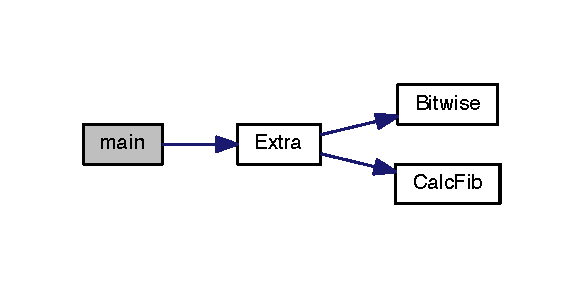
\includegraphics[width=280pt]{_expression_calc_8c_ae66f6b31b5ad750f1fe042a706a4e3d4_cgraph}
\end{center}
\end{figure}



\hypertarget{_r_e_a_d_m_e_8md}{\section{Last\+Badge/\+Developing\+Computer\+Programming/\+R\+E\+A\+D\+M\+E.md File Reference}
\label{_r_e_a_d_m_e_8md}\index{Last\+Badge/\+Developing\+Computer\+Programming/\+R\+E\+A\+D\+M\+E.\+md@{Last\+Badge/\+Developing\+Computer\+Programming/\+R\+E\+A\+D\+M\+E.\+md}}
}

%--- End generated contents ---

% Index
\newpage
\phantomsection
\addcontentsline{toc}{chapter}{Index}
\printindex

\end{document}
